\subsection{Server und Broker}\label{subsec: Server} \todo{anpassen}
Als Server wird ein Versuch aufgebaut, in dem ein Raspberry Pi  der 4 Generation als inhouse Server verwendet wird. Auf dem Markt sind gibt es unzählige kostenlose Online-MQTT-Broker, bei diesen aber Zuverlässigkeit und Diskretion nicht den Projekt Bedingungen entspricht. Daher kann entweder eine teure Cloud-Server Lösung online gekauft oder ein eigener Broker eingerichtet werden. In diesem Projekt wird auf das Raspberry ein MQTT Broker Installiert, dazu wird der viel verbreitete Mosquitto Broker getestet. Der Mosquitto Broker ist Open Source von Eclipse und befindet sich bereits in den Repositoris der betreffenden Distribution. Möglich ist aber auch direkt den Server von openHAB (folglich: Kapitel \ref{subsubsec: Smart-Home Plattform}) zu verwenden.
\paragraph{Inbetriebnahme Raspi}
In diesem Artikel wird erklärt wie das Raspi in Betrieb genommen wird und ins gleiche Subnetz wie der Host verbunden wird. Nach dieser Inbetriebnahme können Befehle einfach mit Secure Shell (ssh) ausgeführt werden. Die Verbindung wird mit dem integrierten Funkchip welcher ab dem Modell Pi 3 vorhanden ist, hergestellt.
Als erstes wird die Micro-SD-Karte des RasPis neu formatiert. Das Betriebssystem Raspian Booster Lite steht \cite{noauthor_download_nodate} zur Verfügung es ist ein Java SE Plattform Produkt und kann unter den Oracle Binary Code Licence Bedingungen verwendet werden. Um das Betriebssystem erfolgreich auf die Micro SD Karte zu flashen wird das Programm Etcher \cite{noauthor_balenaetcher_nodate} verwendet. Um die Secure Shell nach dem Boot Vorgang zu benutzen wird ein leeres Textdokument im Boot Ordner erstellt mit dem Namen "ssh", ohne Endung ".txt". Danach können Netzwerkzugangsdaten in einem weiteren Textdokument "wpa\_supplicant.conf " mit den lokalen Wlan Zugangsdaten erstellt werden, siehe nachfolgende Abbildung \ref{pic: wpasupplicant}. 

\begin{figure}[H]
	\centering
	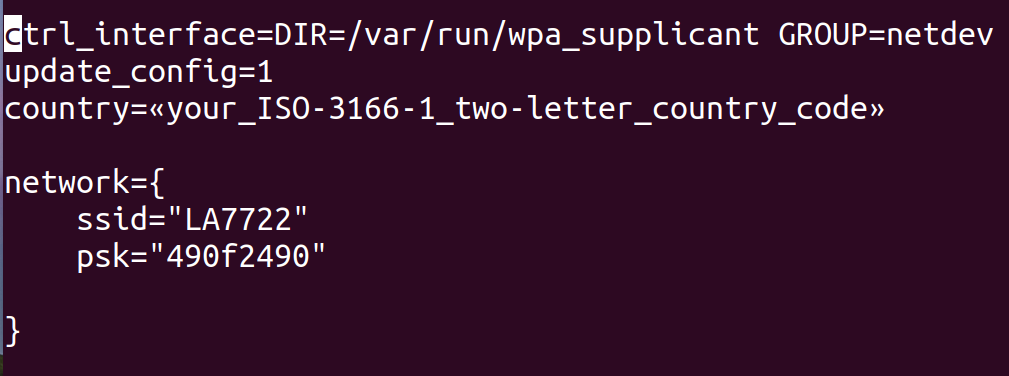
\includegraphics[width=0.75\textwidth]{graphics/WPAsupplicant.png}
	\caption{Konfiguration File wpa supplicant}
	\label{pic: wpasupplicant}
\end{figure}

Im Lokalen Netzwerk kann nun kontrolliert werden ob sich ein Gerät also das RasPi verbunden hat und die IP-Adresse wird angezeigt. Mit dem Konsolenbefehl ssh pi@192.168. . . ist ein Login auf das RasPi möglich. Der Benutzername lautet pi und das Passwort raspberry. Die Netzwerkzugangsdaten können mit dem Befehl \\ 
'sudo nano /etc/wpa\_supplicant/wpa\_supplicant.conf'  geändert werden.


\paragraph{Mosquitto}
Als erstes, vor einer neuen Installation, soll das System des Raspberrys auf den neusten Stand gebracht werden, dies kann mit dem Befehl 'sudo apt-get update' geschehen.
Mit dem Befehl 'sudo apt-get install mosquitto' wird der Server installiert und ist sofort einsatzbereit \cite{noauthor_eigener_nodate}. Beim installierten Mosquitto-Broker kann nun in einem Konfigurationsfile, Benutzer und Passwort generiert werden. Standartkonfigurationen sind durch die Installation bereits angelegt worden, wobei zusätzliche Einstellungen als Datei im Verzeichnis unter '/etc/mosquitto/conf.d/' abgelegt werden. Mit dem Befehl 'sudo mosquitto\_passwd -c /etc/mosquitto/mqttpasswd systemreader' wird der Benutzer Systemreader erstellt, das Passwort muss anschliessend festgelegt werden. Es wurde noch ein weiterer Benutzer ravpi01 erstellt, wobei dann im Befehl zur Benutzererstellung das '-c' weggelassen werden muss sonst wird der erste Benutzer überschrieben. Die erstellten Benutzer können unter dem Befehl 'sudo nano /etc/mosquitto/mqttpasswd' bearbeitet werden siehe Abbildung  \ref{pic: KonfigMosquitto}.

\begin{figure}[H]
	\centering
	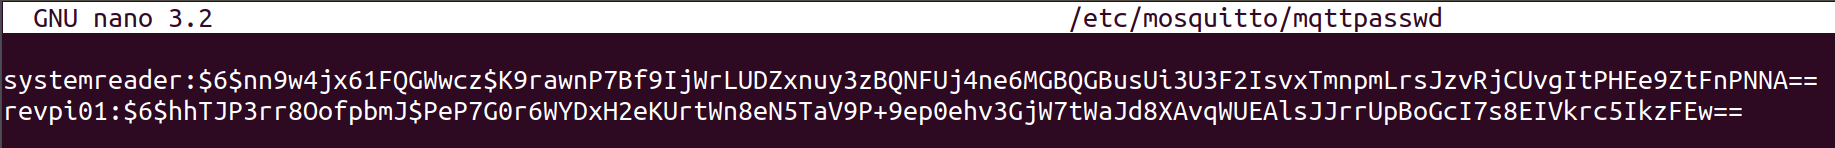
\includegraphics[width=0.75\textwidth]{graphics/MosquittoKonfig.png}
	\caption{Konfiguration File Mosquitto}
	\label{pic: KonfigMosquitto}
\end{figure}

Um Benutzern eine Berechtigung auf bestimmte Topics zu geben, wird eine weitere Datei erstellt. Topics helfen Daten Stream auseinander zu halten. So können zum Beispiel Daten von einem Temperatursensor, der im Wohnzimmer misst, genau von den Daten des Sensors, welcher die Temperatur im Schlafzimmer misst, unterschieden werden. Die Datei wird mit dem Befehl '/etc/mosquitto/user.acl' angelegt. 
In Abbildung \ref{pic: useracl} ist dem systemreader die Berechtigung gegeben, dass er alles lesen darf und dem Benutzer revpi01, dass er nur in nur in 'temperatursensor1/revpi01/' schreiben und lesen darf. 

\begin{figure}[H]
	\centering
	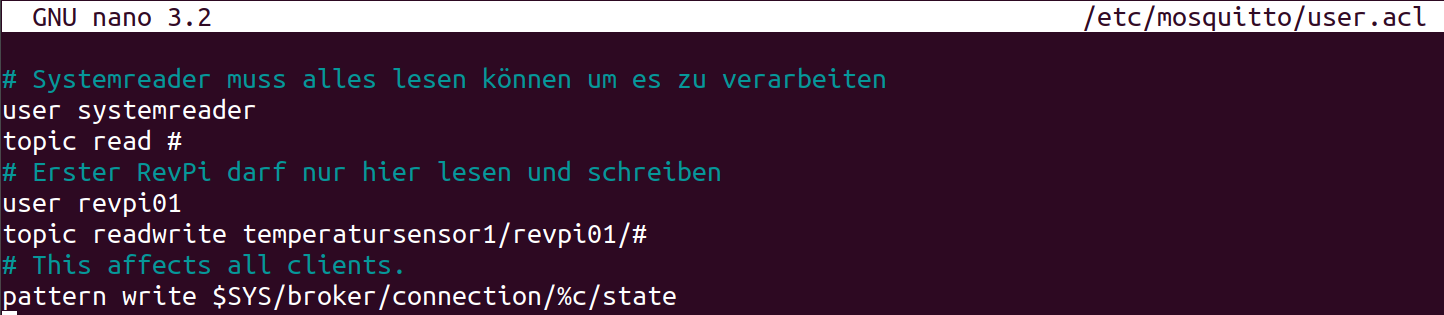
\includegraphics[width=0.75\textwidth]{graphics/useracl.png}
	\caption{Konfiguration Topic Berechtigungen}
	\label{pic: useracl}
\end{figure}

Zu den beiden erstellten Dateien werden nun dem Mosquitto Konfigurationen hinzugefügt, mit dem Befehl 'sudo nano /etc/mosquitto/conf.d/secure.conf', Es öffnet sich ein File, bei welchem der Text wie in Abbildung \ref{pic: secureconf} verfasst werden kann.

\begin{figure}[H]
	\centering
	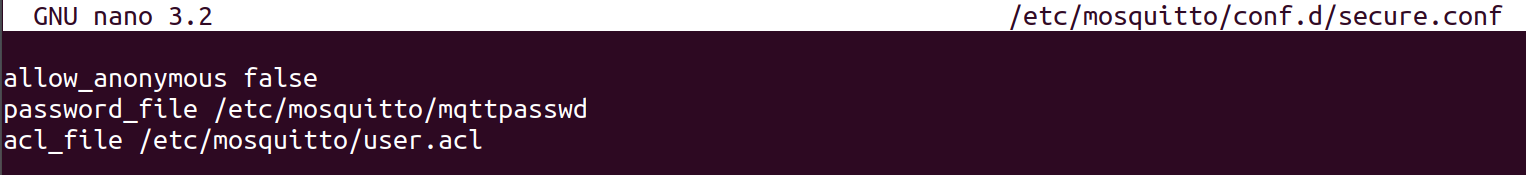
\includegraphics[width=0.75\textwidth]{graphics/MosquittoSecureConf.png}
	\caption{Konfigurationen File hinzufügen}
	\label{pic: secureconf}
\end{figure}

Der Mosquitto-Server soll nach den Konfigurationen neu gestartet werden. Mit dem Befehl 'sudo systemctl restart mosquitto' wird ein reboot durchgeführt und anschliessend kann mit dem Befehl 'sudo systemctl status mosquitto' den Staus des Mosquitto-Servers geprüft werden. Läuft das System korrekt, ist ein grüner Punkt ersichtlich, folglich Abbildung \ref{pic: mosquittoStatus}.

\begin{figure}[H]
	\centering
	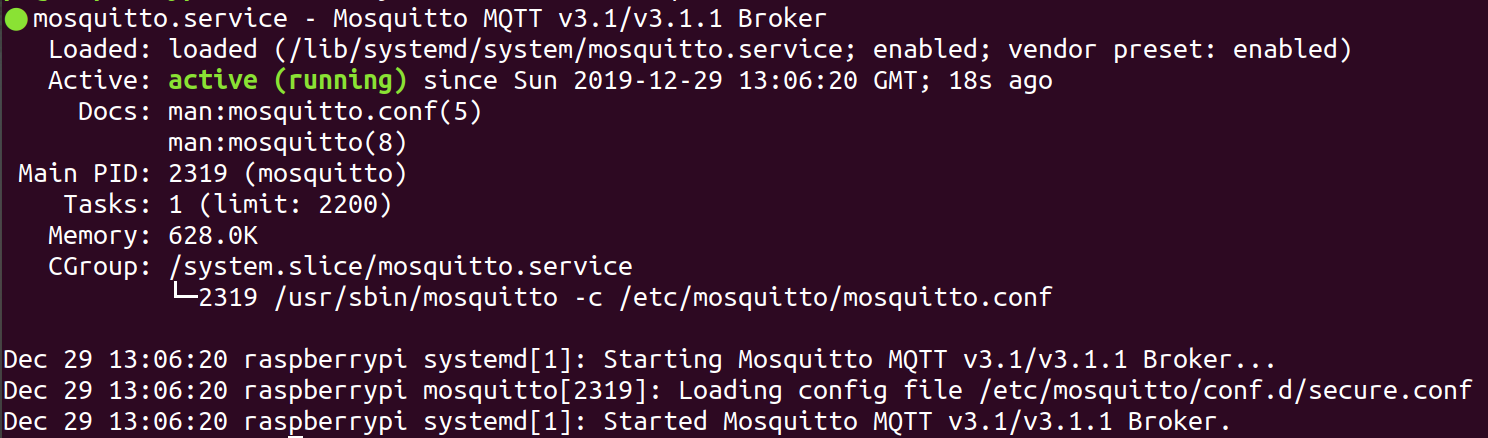
\includegraphics[width=0.75\textwidth]{graphics/MosquittoStatus.png}
	\caption{Mosquitto Status}
	\label{pic: mosquittoStatus}
\end{figure}


